%класс документа, А4, шрифт
\documentclass[reprint, amsmath, amssymb, aps,]{revtex4-2}
%\documentclass[a4paper,12pt]{article}

\usepackage[T2A]{fontenc} %кодировка
\usepackage[utf8]{inputenc} %кодировка исходного текста
\usepackage[english, russian]{babel} %локализация и переносы

%математика
\usepackage{amsmath, amsfonts, amssymb, amsthm, mathtools}

%графика
\usepackage{graphicx}
\DeclareGraphicsExtensions{.pdf,.png,.jpg}
\usepackage{wrapfig} %обтекание фигур

\usepackage{multirow}
\usepackage{dcolumn}% Align table columns on decimal point
\usepackage{bm}% bold math
\usepackage{caption}

\begin{document}
\title{Практические задачи по курсу: Методы анализа распределений данных с тяжёлыми хвостами. Вариант: 7}



\author{Васильев Михаил Владимирович}
\affiliation{%
 Студент 5 курса факультета ФРКТ\\
}%

\collaboration{Московский физико-технический институт}%\noaffiliation

\date{16 декабря 2023 г.}% It is always \today, today,
             %  but any date may be explicitly specified
             

%\begin{abstract}
%\textbf{В работе исследуются:} абсолютная активность радиоактивного препарата $Co^{60}$ с использованием каскадного перехода $\gamma$ квантов при его распаде.
%\begin{description}
%\item[Оборудование]
%высоковольтный стабилизированный выпрямитель, сцинтиллятор, кристалл йодистого натрия NaI(Ti), формирователь импульсов, %схема совпадений, пересчётный прибор, образец $Co^{60}$
%\end{description}
%\end{abstract}

\maketitle

\section{Data}
Данные взяты из массив данных моделирования случайных графов, полученных с помощью моделей предпочтительного присоединения и кластерного присоединения с разными параметрами для анализа. Данные представляют из себя стобец Excel размером 500 значений. 


\section{Exercise 1}
Постановка задачи:

Сгенерировать распределение Фреше с параметром $\gamma = 1.5$.


\begin{equation} \label{Функция распределения Фреше}
F(x) = exp(-(\gamma x)^{-1/\gamma} 1(x>0))
\end{equation}


\begin{center}
\centering 
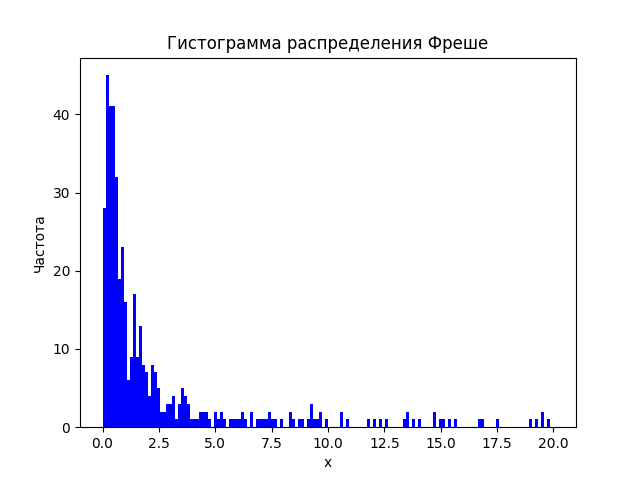
\includegraphics[scale=0.6]{Exercise1.png}
\captionof{figure}{Распределение Фреше}
\end{center}

\section{Exercise 2}
Постановка задачи:
Рассчитать следующую статистику:
\begin{equation} \label{Ex 2}
R_{n}(p) = \frac{M_{n}(p)}{S_{n}(p)}, n\geq 1, p > 0
\end{equation}

\begin{equation} \label{Ex 2.1}
M_{n}(p) = max(|X_{1}|^{p}, ..., |X_{n}|^{p}),
\end{equation}

\begin{equation} \label{Ex 2.2}
S_{n}(p) = |X_{1}|^{p}+...+|X_{n}|^{p}
\end{equation}

sample: $X^{n}=X_{1}, ..., X_{n}$ для $n=1, 2,...$


\begin{center}
\centering 
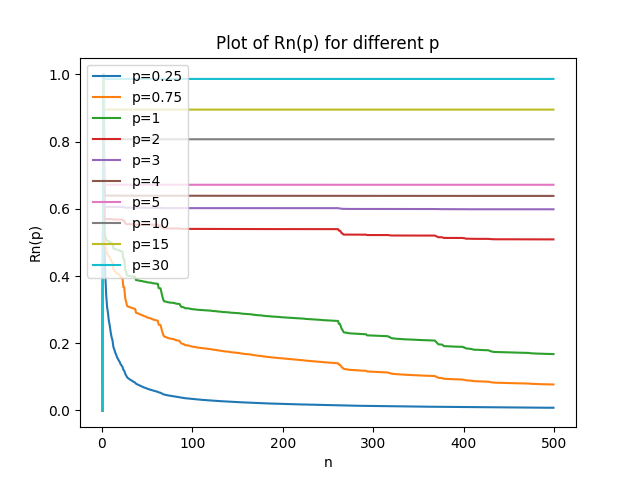
\includegraphics[scale=0.6]{Exercise2.png}
\captionof{figure}{Зависимость отношшения максимума к сумме элементов для различных значений хвостового индекса}
\end{center}

По итогам исследования можно сказать, 
Для $p \in \lbrace 0.25, 0.75, 1 \rbrace $ $R_{n}(p)$ по всей видимости стремиться к нулю при возрастании n.
Для $p \in \lbrace 2, 3, 4, 5, 10, 15, 30 \rbrace $ $ Rn(p)$ по всей видимости стремиться к положительной константе при возрастании n.

Вывод: $E|X|^{p} < \infty$ для $p \leqslant 1$ только, $E|X|^{p} = \infty$ для $p > 1$.


\section{Exercise 3}
Постановка задачи:
Построить QQ-plot для упорядоченных данных для распределений: нормального, логнормального, экспоненциального и Парето общего.

На графиках представлен QQ-plot, где красная линия $y=x$

\begin{center}
\centering 
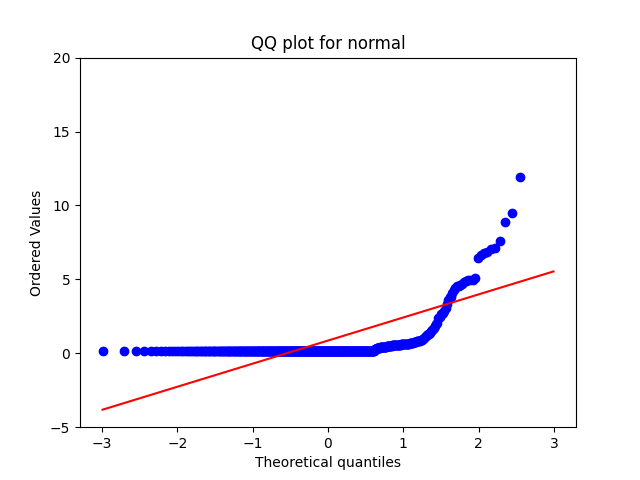
\includegraphics[scale=0.6]{Exercise31.png}
\captionof{figure}{QQ-plot для нормального распределения}
\end{center}
Как видно нормальное распределение не подходит для выборки.

\begin{center}
\centering 
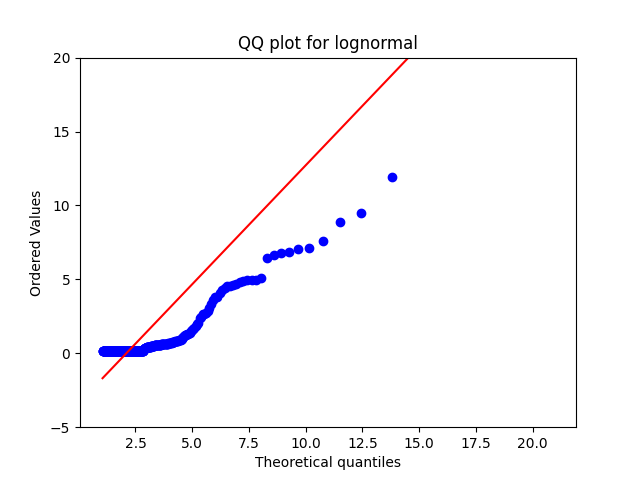
\includegraphics[scale=0.6]{Exercise32.png}
\captionof{figure}{QQ-plot для логнормального распределения}
\end{center}
Как видно логнормальное распределение не подходит для выборки.

\begin{center}
\centering 
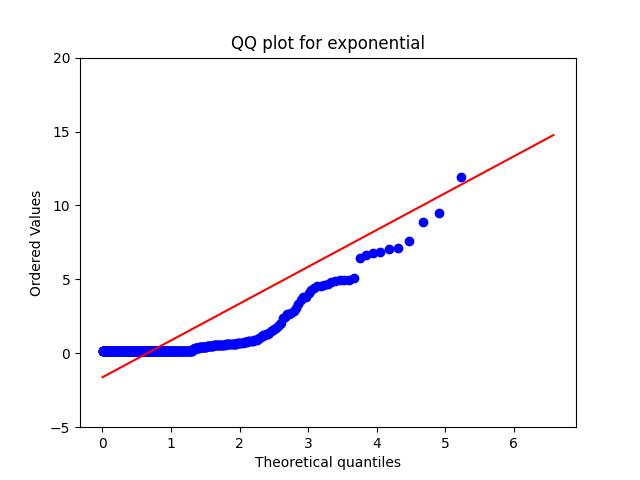
\includegraphics[scale=0.6]{Exercise33.png}
\captionof{figure}{QQ-plot для экспоненциального распределения}
\end{center}

Как видно экспоненциальное распределение не подходит для выборки.

\begin{center}
\centering 
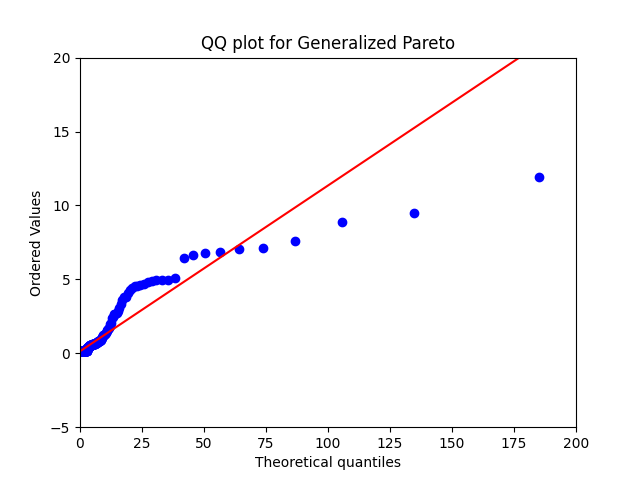
\includegraphics[scale=0.6]{Exercise34.png}
\captionof{figure}{QQ-plot для Парето обобщённого}
\end{center}

Как видно Парето обобщённое распределение не подходит для выборки.

\begin{center}
\centering 
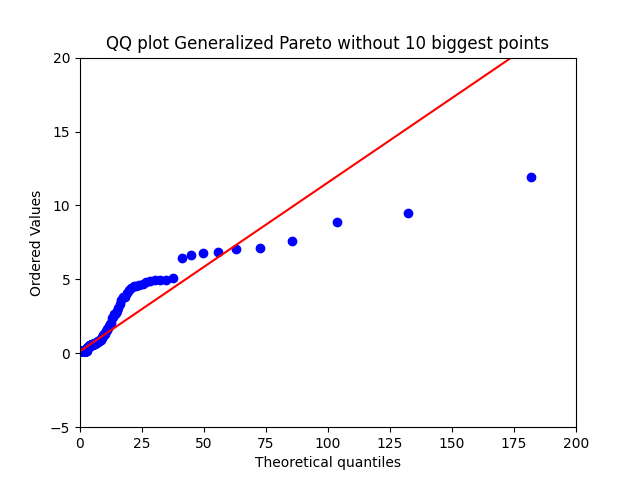
\includegraphics[scale=0.6]{Exercise35.png}
\captionof{figure}{QQ-plot для Парето обобщённого распределения без наибольших 10 точек}
\end{center}
Как видно убирание наибольших значений из выборки слабо влияет на QQ-plot.

Вывод: ни одно из распределений не подходит для описания выборки, убирание наибольших значений выборки не имеет смысла.


\section{Exercise 4}
Постановка задачи:
Построить график mean excess function.

\begin{equation} \label{Ex 4}
e_{n}(u)= \sum_{i=1}^n (X_{i}-u)1(X_{i}>u)/ \sum_{i=1}^n 1(X_{i}>u)
\end{equation}


\begin{center}
\centering 
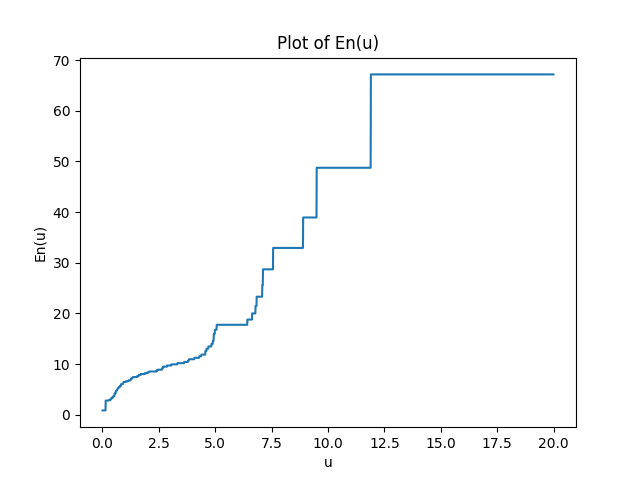
\includegraphics[scale=0.6]{Exercise4.png}
\captionof{figure}{График для mean excess function}
\end{center}

Видно что для больших u график $e_{n}(u)$ стремится к бесконечности, что означает, что распределение принадлежит к классу распределений с тяжёлыми хвостами.

Вывод: распределение имеет тяжёлые хвосты.

\section{Exercise 5}
Постановка задачи:
Having the empirical or generated data $X_{n} = \lbrace X_{1}, ...,X_{n} \rbrace$ reorder the data as $X(1) \leq X(2) \leq ... \leq X(n)$.
Calculate and compare the following estimates of the tail index of your data. Investigate the sign of an estimate and make conclusion regarding the heavy tails.

\begin{center}
\centering 
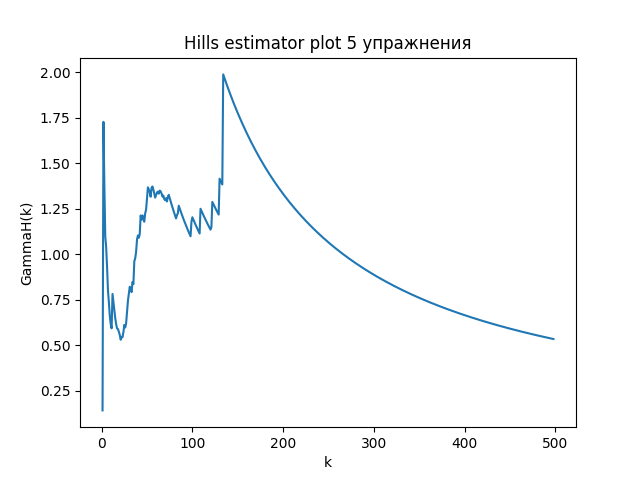
\includegraphics[scale=0.6]{Exercise51.png}
\captionof{figure}{Hills estimator plot}
\end{center}

\begin{center}
\centering 
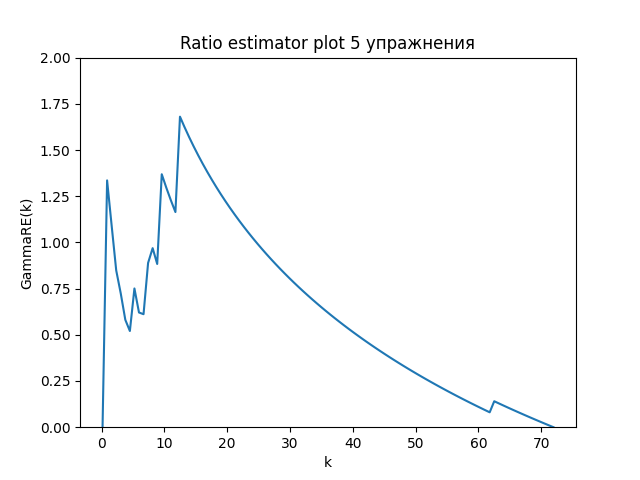
\includegraphics[scale=0.6]{Exercise52.png}
\captionof{figure}{Ratio estimator plot}
\end{center}

\begin{center}
\centering 
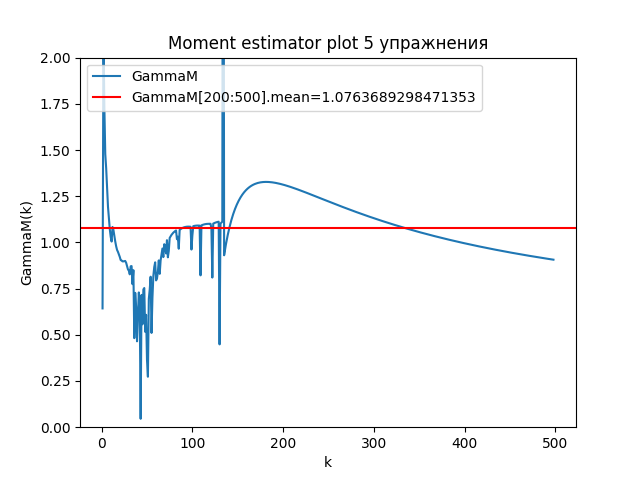
\includegraphics[scale=0.6]{Exercise53.png}
\captionof{figure}{Moment estimator plot}
\end{center}

\begin{center}
\centering 
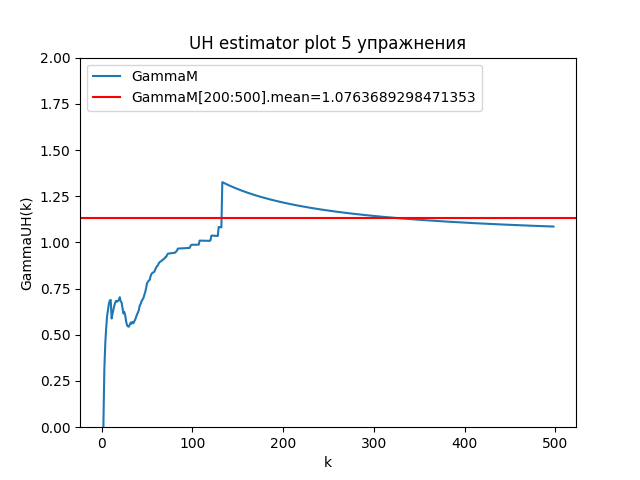
\includegraphics[scale=0.6]{Exercise54.png}
\captionof{figure}{UH estimator plot}
\end{center}

\begin{center}
\centering 
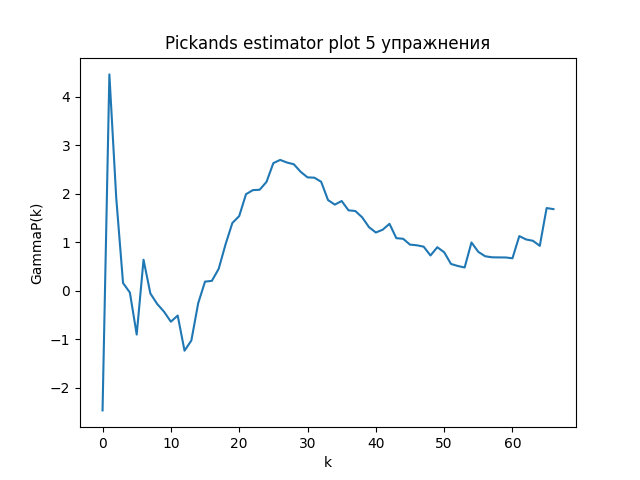
\includegraphics[scale=0.6]{Exercise55.png}
\captionof{figure}{Pickands estimator plot}
\end{center}

Из графиков видно, что оценки Hill, Ratio и Pickands на предоставленных данных работают плохо. Тогда как оценки Moment и UH стабилизируются между 200 и 500 значением выборки. При взятии среднего по этим оценкам между 200 и 500 элементом выборки получаются значения 1.0763 и 1.131 соответственно.

Вывод: по всей видимости хвостовой индекс можно положить примерно равным $\gamma \thickapprox 1.1$.    

\section{Exercise 6}
Постановка задачи:
Вывести эстиматор Хилла с доверительным интервалом.

\begin{center}
\centering 
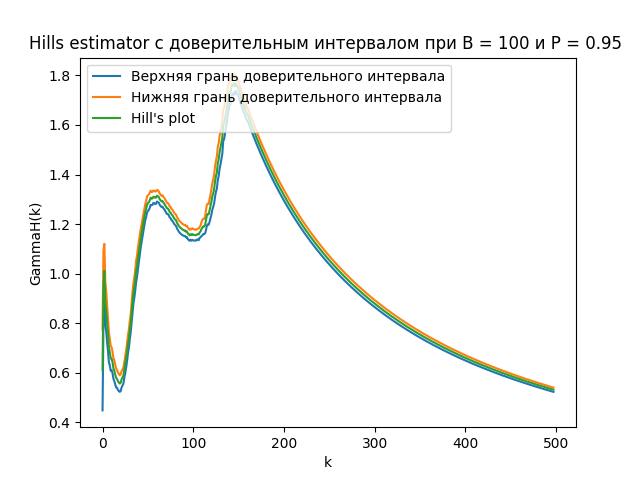
\includegraphics[scale=0.6]{Exercise6.png}
\captionof{figure}{Hills estimator with confidence interval}
\end{center}



\end{document}